\documentclass[a4paper,12pt]{report}
\usepackage[toc,page]{appendix}
\usepackage{amsmath}
\usepackage{float}
\usepackage{graphicx}
\usepackage{subfig}
\usepackage{amssymb}
\usepackage{geometry}
\usepackage{array}
\usepackage{tcolorbox}

\usepackage{setspace}
 \geometry{
 a4paper,
 total={170mm,257mm},
 left=20mm,
 top=20mm,
 }
\usepackage{tikz}
\usepackage{pgfplots}
\usetikzlibrary{shapes, arrows.meta, decorations.pathreplacing, positioning, petri, fit, calc}
\tikzstyle{startstop} = [circle, minimum size=1cm ,text centered, draw=black]
\tikzstyle{neuron} = [circle, minimum size=1cm ,text centered, draw=red, fill=gray!30]
\tikzstyle{neuronEll} = [ellipse, minimum size=1cm ,text centered, text width=2cm, draw=red, fill=gray!30]
\tikzstyle{process} = [rectangle, minimum width=2cm, minimum height=0.5cm, text centered, text width=3cm, draw=black, fill=blue!30]
\tikzstyle{detail} = [rectangle, minimum width=1.5cm, minimum height=0.5cm, text justified, text width=2.6cm, fill=white!30]
\tikzstyle{smalldetail} = [rectangle, minimum width=2cm, minimum height=1cm, text centered, text width=2cm]
\tikzstyle{largedetail} = [rectangle, minimum width=3cm, minimum height=1cm, text centered, text width=4cm, fill=white!30]
\tikzstyle{box} = [rectangle, minimum width=5cm, minimum height=9cm, text centered, text width=4cm, draw=black, fill=white!30]

\usepackage[utf8]{inputenc}

% Default fixed font does not support bold face
\DeclareFixedFont{\ttb}{T1}{txtt}{bx}{n}{10} % for bold
\DeclareFixedFont{\ttm}{T1}{txtt}{m}{n}{10}  % for normal

% Custom colors
\usepackage{color}
\definecolor{deepblue}{rgb}{0,0,0.5}
\definecolor{deepred}{rgb}{0.6,0,0}
\definecolor{deepgreen}{rgb}{0,0.5,0}

\usepackage{listings}

% Python style for highlighting
\newcommand\pythonstyle{\lstset{
language=Python,
basicstyle=\ttm,
otherkeywords={self},             % Add keywords here
keywordstyle=\ttb\color{deepblue},
emph={MyClass,__init__},          % Custom highlighting
emphstyle=\ttb\color{deepred},    % Custom highlighting style
stringstyle=\color{deepgreen},
frame=tb,                         % Any extra options here
showstringspaces=false            % 
}}


% Python environment
\lstnewenvironment{python}[1][]
{
\pythonstyle
\lstset{#1}
}
{}

% Python for external files
\newcommand\pythonexternal[2][]{{
\pythonstyle
\lstinputlisting[#1]{#2}}}

% Python for inline
\newcommand\pythoninline[1]{{\pythonstyle\lstinline!#1!}}


\begin{document}
\tableofcontents

\title{Neural Networks and Back Propagation}
\begin{itemize}
\textbf{Back propagation:}
\item requires labeled training data
\item the learning time scales well (it is very slow in network with multiple hidden layers).
\item It can get stuck in poor local minima
\end{itemize}
\maketitle
\part{Week 5}
\section{Pro and Cons}
\begin{table}[H]
\begin{tabular}{|l|l|}
\hline
\hline
Advantages of NN & Disadvantages \\
\hline
\textbf{+} Can represent non-linear boundary &  \textbf{+} Gradient descent is not guaranteed \\
& to reach a global optimum \\
\textbf{+} Fast feed forward architecture &  \textbf{+} We do not know the optimal architecture \\
& (Nbr of inputs/hidden nodes/layers/output nodes) \\
& \textbf{+} setting the adjustable parameter learning rate \\
\hline
\end{tabular}
\end{table}
Note that it is sometimes preferable to stop training early for better generalization performance. Generalization means performance on unseen input data - if you train too long, you can often get over-fitting. By stopping the training earlier, one hopes that the network will have learned the broad rules of the problem.
\section{Cost function}
Let's consider a Neural Network with 4 layers. In this example with 2 features, one could use logistic regression with polynomial terms:

\begin{figure}[H]
        \centering
        \resizebox {4in} {!} {
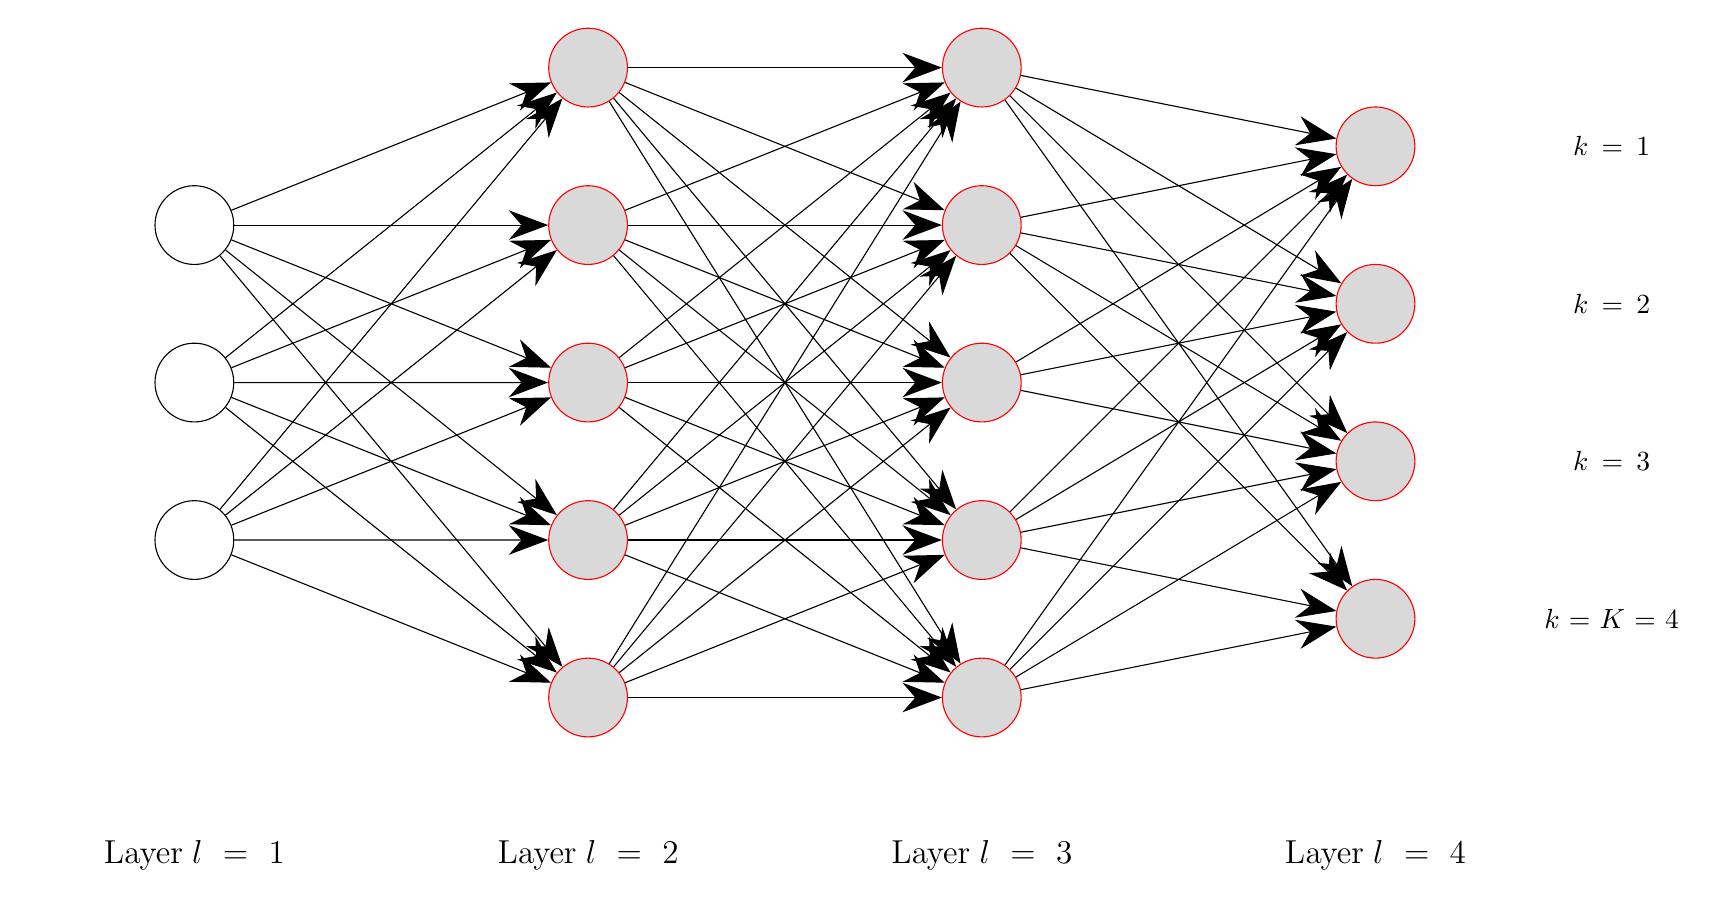
\begin{tikzpicture}[node distance=4cm]
\node (x1) [startstop] {};
\node (x2) [startstop, below of=x1, xshift=0cm, yshift=2cm] {};
\node (x3) [startstop, below of=x2, xshift=0cm, yshift=2cm] {};
\node (layer1) [largedetail, below of=x2, xshift=0cm, yshift=-2cm] {\large{Layer $l=1$}};
\node (a11) [neuron, below of=x1, xshift=5cm, yshift=6cm] {};
\node (a12) [neuron, below of=a11, xshift=0cm, yshift=2cm] {};
\node (a13) [neuron, below of=a12, xshift=0cm, yshift=2cm] {};
\node (a14) [neuron, below of=a13, xshift=0cm, yshift=2cm] {};
\node (a15) [neuron, below of=a14, xshift=0cm, yshift=2cm] {};
\node (layer2) [largedetail, below of=layer1, xshift=5cm, yshift=4cm] {\large{Layer $l=2$}};
\node (a21) [neuron, below of=a11, xshift=5cm, yshift=4cm] {};
\node (a22) [neuron, below of=a21, xshift=0cm, yshift=2cm] {};
\node (a23) [neuron, below of=a22, xshift=0cm, yshift=2cm] {};
\node (a24) [neuron, below of=a23, xshift=0cm, yshift=2cm] {};
\node (a25) [neuron, below of=a24, xshift=0cm, yshift=2cm] {};
\node (layer3) [largedetail, below of=layer2, xshift=5cm, yshift=4cm] {\large{Layer $l=3$}};
\node (a31) [neuron, below of=a21, xshift=5cm, yshift=3cm] {};
\node (a32) [neuron, below of=a31, xshift=0cm, yshift=2cm] {};
\node (a33) [neuron, below of=a32, xshift=0cm, yshift=2cm] {};
\node (a34) [neuron, below of=a33, xshift=0cm, yshift=2cm] {};
\node (outputk1) [smalldetail, below of=a31, xshift=3cm, yshift=4cm] {$k=1$};
\node (outputk2) [smalldetail, below of=outputk1, xshift=0cm, yshift=2cm] {$k=2$};
\node (outputk3) [smalldetail, below of=outputk2, xshift=0cm, yshift=2cm] {$k=3$};
\node (outputk4) [smalldetail, below of=outputk3, xshift=0cm, yshift=2cm] {$k=K=4$};
\node (layer4) [largedetail, below of=layer3, xshift=5cm, yshift=4cm] {\large{Layer $l=4$}};
\draw[-{Stealth[length=5mm]}] (x1) -- (a11);
\draw[-{Stealth[length=5mm]}] (x1) -- (a12);
\draw[-{Stealth[length=5mm]}] (x1) -- (a13);
\draw[-{Stealth[length=5mm]}] (x1) -- (a14);
\draw[-{Stealth[length=5mm]}] (x1) -- (a15);
\draw[-{Stealth[length=5mm]}] (x2) -- (a11);
\draw[-{Stealth[length=5mm]}] (x2) -- (a12);
\draw[-{Stealth[length=5mm]}] (x2) -- (a13);
\draw[-{Stealth[length=5mm]}] (x2) -- (a14);
\draw[-{Stealth[length=5mm]}] (x2) -- (a15);
\draw[-{Stealth[length=5mm]}] (x3) -- (a11);
\draw[-{Stealth[length=5mm]}] (x3) -- (a12);
\draw[-{Stealth[length=5mm]}] (x3) -- (a13);
\draw[-{Stealth[length=5mm]}] (x3) -- (a14);
\draw[-{Stealth[length=5mm]}] (x3) -- (a15);
\draw[-{Stealth[length=5mm]}] (a11) -- (a21);
\draw[-{Stealth[length=5mm]}] (a11) -- (a22);
\draw[-{Stealth[length=5mm]}] (a11) -- (a23);
\draw[-{Stealth[length=5mm]}] (a11) -- (a24);
\draw[-{Stealth[length=5mm]}] (a11) -- (a25);
\draw[-{Stealth[length=5mm]}] (a12) -- (a21);
\draw[-{Stealth[length=5mm]}] (a12) -- (a22);
\draw[-{Stealth[length=5mm]}] (a12) -- (a23);
\draw[-{Stealth[length=5mm]}] (a12) -- (a24);
\draw[-{Stealth[length=5mm]}] (a12) -- (a25);
\draw[-{Stealth[length=5mm]}] (a13) -- (a21);
\draw[-{Stealth[length=5mm]}] (a13) -- (a22);
\draw[-{Stealth[length=5mm]}] (a13) -- (a23);
\draw[-{Stealth[length=5mm]}] (a13) -- (a24);
\draw[-{Stealth[length=5mm]}] (a13) -- (a25);
\draw[-{Stealth[length=5mm]}] (a14) -- (a21);
\draw[-{Stealth[length=5mm]}] (a14) -- (a22);
\draw[-{Stealth[length=5mm]}] (a14) -- (a23);
\draw[-{Stealth[length=5mm]}] (a14) -- (a24);
\draw[-{Stealth[length=5mm]}] (a14) -- (a25);
\draw[-{Stealth[length=5mm]}] (a15) -- (a21);
\draw[-{Stealth[length=5mm]}] (a15) -- (a22);
\draw[-{Stealth[length=5mm]}] (a15) -- (a23);
\draw[-{Stealth[length=5mm]}] (a15) -- (a24);
\draw[-{Stealth[length=5mm]}] (a15) -- (a25);
\draw[-{Stealth[length=5mm]}] (a21) -- (a31);
\draw[-{Stealth[length=5mm]}] (a21) -- (a32);
\draw[-{Stealth[length=5mm]}] (a21) -- (a33);
\draw[-{Stealth[length=5mm]}] (a21) -- (a34);
\draw[-{Stealth[length=5mm]}] (a22) -- (a31);
\draw[-{Stealth[length=5mm]}] (a22) -- (a32);
\draw[-{Stealth[length=5mm]}] (a22) -- (a33);
\draw[-{Stealth[length=5mm]}] (a22) -- (a34);
\draw[-{Stealth[length=5mm]}] (a23) -- (a31);
\draw[-{Stealth[length=5mm]}] (a23) -- (a32);
\draw[-{Stealth[length=5mm]}] (a23) -- (a33);
\draw[-{Stealth[length=5mm]}] (a24) -- (a31);
\draw[-{Stealth[length=5mm]}] (a24) -- (a32);
\draw[-{Stealth[length=5mm]}] (a24) -- (a33);
\draw[-{Stealth[length=5mm]}] (a24) -- (a34);
\draw[-{Stealth[length=5mm]}] (a25) -- (a31);
\draw[-{Stealth[length=5mm]}] (a25) -- (a32);
\draw[-{Stealth[length=5mm]}] (a25) -- (a33);
\draw[-{Stealth[length=5mm]}] (a25) -- (a34);
\end{tikzpicture}
}
\end{figure}

\begin{itemize}
\item Given a set of training examples are $\{(x^{(1)},y^{(1)}),(x^{(2)},y^{(2)}),.....,(x^{(m)},y^{(m)})  \} $ ($i$=i$^{\mathrm{th}}$ training example).
\begin{itemize}
\item $L$ :  number of layers in network (here $L=4$)
\item $s_l$ : total number of units (not including the bias unit) in layer $l$ ($s_1=3, ..., s_4=s_L=4)$
\item $K$ : number of output units (classes)
\end{itemize}
\end{itemize}

\subsection{Binary vs. Multiclass}
\begin{itemize}
\item For Binary Classification $y \in \{0,1\}$
\begin{itemize}
\item $s_L = 1$
\item $K=1$ (1 ouput unit)
\item $h_{\Theta}(x) \in \mathbb{R}$
\end{itemize}
\end{itemize}
\resizebox {2in} {!} {
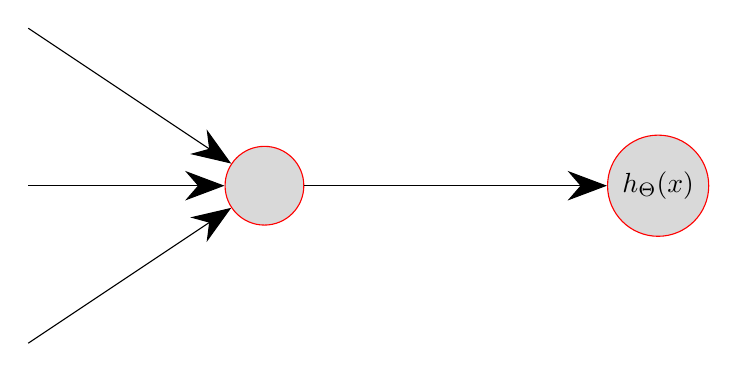
\begin{tikzpicture}[node distance=4cm]
\node (output) [neuron] {};
\node (h) [neuron, below of=output, xshift=5cm, yshift=4cm] {$h_{\Theta}(x)$};
\draw [-{Stealth[length=5mm]}] (-3,2) -- (output);
\draw [-{Stealth[length=5mm]}] (-3,0) -- (output);
\draw [-{Stealth[length=5mm]}] (-3,-2) -- (output);
\draw [-{Stealth[length=5mm]}] (output) -- (h);
\end{tikzpicture}}  \\

\begin{itemize}
\item For Multiclass classification
\begin{itemize}
\item $K$ output units ($y \in \mathbb{R}^{K}$) \\
for example 4 classes: $\left[\begin{smallmatrix}1\\0\\0\\0 \end{smallmatrix} \right], \left[\begin{smallmatrix}0\\1\\0\\0 \end{smallmatrix} \right], \left[\begin{smallmatrix}0\\0\\1\\0 \end{smallmatrix} \right], \left[\begin{smallmatrix}0\\0\\0\\1 \end{smallmatrix} \right]$
\item $h_{\Theta}(x)_k$ is the hypothesis that results in the $k^{\mathrm{th}}$ output
\item $s_L = K$ where $K \geq 3$  
\end{itemize}
\end{itemize}

\subsection{Calculate Cost function}
\begin{itemize}
\item \textbf{Logistic regression}
\end{itemize}
\begin{align*}
J(\theta) = -\frac{1}{m} \left[\sum_{i=1}^m y^{(i)} \mathrm{log}(h_{\theta}(x^{(i)})) + (1- y^{(i)}) \mathrm{log}(1-h_{\theta}(x^{(i)}))\right] + \frac{\lambda}{2m} \sum_{j=1}^n \theta_j ^2
\end{align*}

\begin{itemize}
\item \textbf{Neural Network}
\end{itemize}
$h_{\Theta}(x) \in \mathbb{R}^K$, where $(h_{\Theta}(x))_k$ is the $k^{\mathrm{th}}$ output.

\begin{align*}
J(\theta) = -\frac{1}{m} \left[\sum_{i=1}^m \sum_{k=1}^K y_k^{(i)} \mathrm{log} [ (h_{\Theta}(x^{(i)}))_k] + (1- y_k^{(i)}) \mathrm{log}[1- \left(h_{\theta}(x^{(i)}) \right)_k ]\right] + \frac{\lambda}{2m} \sum_{l=1}^{L-1}\sum_{i=1}^{s_l}\sum_{j=1}^{s_{l+1}} \left(\Theta_{ij} ^{(l)} \right)^2
\end{align*}
\begin{itemize}
\item 1st term: sum of the logistic regression costs calculated for each unit in the output layer, for each training example
\item 2nd term is called the weight decay term\footnote{A most popular regularization method is known as weight decay: $1/2 \sum_k w_k^2$ (sum of all squared weights). One weakness of the weight decay method is that it is not able to drive small iirelevant weights to zero, which may results in many small weights}: sum of all the individual $\Theta$'s in the entire network. \\
Note that the $i$ in $\sum_{i=1}^{s_l} $ does not refer to the training example 
\end{itemize}

\section{Minimization of the Cost Function}
We need to compute the cost function, and minimize it: $\mathrm{min}_{\Theta} J(\Theta)$:
\begin{align*}
\frac{\partial}{\partial \Theta_{ij} ^{(l)}} J(\Theta) \mathrm{\ with \ } \Theta_{ij} ^{(l)} \in \mathbb{R}
\end{align*}
\subsection{Compute Gradient}
Let's start with a system with one training example $(x,y)$:
\\
\begin{itemize}
\item \textbf{Forward Propagation}
\end{itemize}
\begin{figure}[H]
\begin{center}$
\begin{array}[m]{r|l}
\resizebox {2in} {!} {
\begin{tikzpicture}[node distance=4cm]
\node (x0) [startstop, below of=x1, xshift=0cm, yshift=4cm] {};
\node (x1) [startstop] {};
\node (x2) [startstop, below of=x1, xshift=0cm, yshift=2cm] {};
\node (x3) [startstop, below of=x2, xshift=0cm, yshift=2cm] {};
\node (layer1) [largedetail, below of=x2, xshift=0cm, yshift=-4cm] {\huge{Layer l=1}};
\node (a01) [neuron, below of=a11, xshift=0cm, yshift=2cm] {};
\node (a11) [neuron, below of=x1, xshift=5cm, yshift=6cm] {};
\node (a12) [neuron, below of=a11, xshift=0cm, yshift=2cm] {};
\node (a13) [neuron, below of=a12, xshift=0cm, yshift=2cm] {};
\node (a14) [neuron, below of=a13, xshift=0cm, yshift=2cm] {};
\node (a15) [neuron, below of=a14, xshift=0cm, yshift=2cm] {};
\node (layer2) [largedetail, below of=layer1, xshift=5cm, yshift=4cm] {\huge{Layer l=2 }};
\node (a21) [neuron, below of=a11, xshift=5cm, yshift=4cm] {};
\node (a22) [neuron, below of=a21, xshift=0cm, yshift=2cm] {};
\node (a23) [neuron, below of=a22, xshift=0cm, yshift=2cm] {};
\node (a24) [neuron, below of=a23, xshift=0cm, yshift=2cm] {};
\node (a25) [neuron, below of=a24, xshift=0cm, yshift=2cm] {};
\node (layer3) [largedetail, below of=layer2, xshift=5cm, yshift=4cm] {\huge {Layer l=3}};
\node (a31) [neuron, below of=a21, xshift=5cm, yshift=3cm] {};
\node (a32) [neuron, below of=a31, xshift=0cm, yshift=2cm] {};
\node (a33) [neuron, below of=a32, xshift=0cm, yshift=2cm] {};
\node (a34) [neuron, below of=a33, xshift=0cm, yshift=2cm] {};
\node (layer4) [largedetail, below of=layer3, xshift=5cm, yshift=4cm] {\huge{Layer l=4 (output)}};
\node (a1) [largedetail, below of=x1, xshift=0cm, yshift=8cm] {\Huge{$a^{(1)}$}};
\node (a2) [largedetail, below of=a11, xshift=0cm, yshift=6cm] {\Huge{$a^{(2)}$}};
\node (a3) [largedetail, below of=a21, xshift=0cm, yshift=6cm] {\Huge{$a^{(3)}$}};
\node (a4) [largedetail, below of=a31, xshift=0cm, yshift=7cm] {\Huge{$a^{(4)}$}};
\end{tikzpicture} }
& 
\begin{array}[b]{rl}
a^{(1)} &= x \\
& \\
a^{(2)} &= g(z^{(2)}) \rightarrow z^{(2)} = \Theta^{(1)} a^{(1)} (\mathrm{\ add\ } a_0 ^{(2)} ) \\
& \\
a^{(3)} &= g(z^{(3)}) \rightarrow z^{(3)} = \Theta^{(2)} a^{(2)} (\mathrm{\ add\ } a_0 ^{(3)} ) \\
& \\
a^{(4)} &= h_{\Theta}(x) = g(z^{(4)}) \rightarrow z^{(4)} = \Theta^{(3)} a^{(3)} \\
& a^{(4)}\mathrm{\  is \  the \ output \ hypothesis \ (vector \  or \  Real)} \\
\end{array}
\end{array}$
\end{center}
\end{figure}


\begin{itemize}
\item \textbf{Back Propagation}
\end{itemize}
Back propagation takes the output $h_{\Theta}(x)$, compares it to $y$ and calculates how wrong the network was, i.e how wrong the $\Theta_{ij} ^l$ were. Using the error calculated on the output layer, we then back-calculate the error associated with each unit from the preceding layer (i.e layer $(L-1)$, ... down to the input layer (where there is obviously no error). These error measurements are then used to calculate the partial derivatives, which gradient descent needs to minimize the cost function. This is repeated until convergence.

\begin{figure}[H]
        \centering
        \resizebox {2in} {!} {
\begin{tikzpicture}[node distance=4cm]
\node (x0) [startstop, below of=x1, xshift=0cm, yshift=4cm] {};
\node (x1) [startstop] {};
\node (x2) [startstop, below of=x1, xshift=0cm, yshift=2cm] {};
\node (x3) [startstop, below of=x2, xshift=0cm, yshift=2cm] {};
\node (layer1) [largedetail, below of=x2, xshift=0cm, yshift=-4cm] {\huge{Layer $l=1$}};
\node (a01) [neuron, below of=a11, xshift=0cm, yshift=2cm] {};
\node (a11) [neuron, below of=x1, xshift=5cm, yshift=6cm] {};
\node (a12) [neuron, below of=a11, xshift=0cm, yshift=2cm] {};
\node (a13) [neuron, below of=a12, xshift=0cm, yshift=2cm] {};
\node (a14) [neuron, below of=a13, xshift=0cm, yshift=2cm] {};
\node (a15) [neuron, below of=a14, xshift=0cm, yshift=2cm] {};
\node (layer2) [largedetail, below of=layer1, xshift=5cm, yshift=4cm] {\huge{Layer $l=2$}};
\node (a21) [neuron, below of=a11, xshift=5cm, yshift=4cm] {};
\node (a22) [neuron, below of=a21, xshift=0cm, yshift=2cm] {};
\node (a23) [neuron, below of=a22, xshift=0cm, yshift=2cm] {};
\node (a24) [neuron, below of=a23, xshift=0cm, yshift=2cm] {};
\node (a25) [neuron, below of=a24, xshift=0cm, yshift=2cm] {};
\node (layer3) [largedetail, below of=layer2, xshift=5cm, yshift=4cm] {\huge{Layer $l=3$}};
\node (a31) [neuron, below of=a21, xshift=5cm, yshift=3cm] {};
\node (a32) [neuron, below of=a31, xshift=0cm, yshift=2cm] {};
\node (a33) [neuron, below of=a32, xshift=0cm, yshift=2cm] {};
\node (a34) [neuron, below of=a33, xshift=0cm, yshift=2cm] {};
\node (layer4) [largedetail, below of=layer3, xshift=5cm, yshift=4cm] {\huge{Layer $l=4$ (output)}};

\node (a1) [largedetail, below of=x1, xshift=0cm, yshift=8cm] {\Huge{$a^{(1)}$}};
\node (a2) [largedetail, below of=a11, xshift=0cm, yshift=6cm] {\Huge{$a^{(2)}$ \\ $\delta^{(2)}$}};
\node (a3) [largedetail, below of=a21, xshift=0cm, yshift=6cm] {\Huge{$a^{(3)}$  \\ $\delta^{(3)}$}};
\node (a4) [largedetail, below of=a31, xshift=0cm, yshift=7cm] {\Huge{$a^{(4)}$  \\ $\delta^{(4)}$}};
\end{tikzpicture}
}\caption{Example of a network [3-5-5-4]. $l$ : layer , $s$: node in that layer}
\end{figure}

\textbf{We define $\delta_j ^{(l)}$ as the "error" of node $j$ in layer $l$}, i.e error of $a_j ^{(l)}$ activation value. It can be shown that (see appendix):
{\center
\fbox{\parbox{\textwidth}{
\begin{itemize}
\item $\delta_j ^{(4)} = a_j ^{(4)} - y_j = [(h_{\Theta}(x))_j - y]$  $\rightarrow$ Vectorized form: $\delta^{4} = a^{4} - y$ \\
($\delta^{4}$, $a^{4}$ and $y$ are all vectors with dimension = Nbr of output unit in layer 4 ($K$) \\
\item $\delta ^{(3)} = \left(\Theta^{(3)} \right)^{T} \delta^{(4)} .* g'\left(z^{(3)} \right) = \left(\Theta^{(3)} \right)^{T} \delta^{(4)} .* ( a^{(3)} .* (1-a^{(3)}))$  \\
\item $\delta ^{(2)} = \left(\Theta^{(2)} \right)^{T} \delta^{(3)} .* g'\left(z^{(2)} \right) = \left(\Theta^{(2)} \right)^{T} \delta^{(3)} .* a^{(2)} .* (1-a^{(2)})$
\end{itemize}
There is no $\delta ^{(1)}$ term for the first layer (input layer).
} } } \\

We can then calculate the derivative of the cost function (for  $\lambda = 0$):
\begin{equation}
\frac{\partial }{\partial \Theta_{ij} ^{(l)}} J(\Theta) = a_j ^{(l)} \delta_i ^{(l+1)}
\end{equation}

\section{Implement Back Propagation Algorithm}
\begin{enumerate}
\item Given a training set of $m$ examples: $\{(x^{(1)}, y^{(1)}),(x^{(2)}, y^{(2)}), .....,(x^{(m)}, y^{(m)}) \} $
\item Set: $\Delta_{ij} ^{(l)} = 0$ for all $l$(layer), $i$, $j$(node) \\
\item For training example $t=1$ thru m:
\begin{itemize}
\item set $a^{(1)} = x^{(t)}$
\item Perform Forward  propagation to compute $a^{(l)}$ for $l=2, 3, ...,L$
\end{itemize} 
\begin{itemize}
\item Using $y^{(t)}$, compute $\delta^{(L)}=a^{(L)} - y^{(t)}$
\item Compute the error node $\delta^{(L-1)}, \delta^{(L-2)}, ...., \delta^{(2)}$  (no $\delta^{(1)}$) using:
\begin{align}
\delta^{(l)} = \left((\Theta^{(l)})^T \delta^{(l+1)}\right).*a^{(l)}.*(1-a^{(l)})
\end{align}
\item Compute accumulators $\Delta$:
\begin{align*}
\Delta_{ij} ^{(l)} := \Delta_{ij} ^{(l)} + a_{j} ^{(l)} \delta_{i} ^{(l+1)} \rightarrow \mathrm{vectorized \  form:\ } \Delta ^{(l)} := \Delta^{(l)} + \delta^{(l+1)} \left(a^{(l)} \right)^{T}
\end{align*}
\item Exit Loop
\end{itemize}
\item Calculate the partial derivatives $D_{ij}^{(l)} = \frac{\partial J(\Theta)}{\partial \Theta_{ij} ^{(l)}}$
\begin{align*}
\begin{split}
D_{ij}^{(l)} :=& \frac{1}{m} \left(\Delta_{ij}^{(l)} + \lambda \Theta_{ij} ^{(l)} \right) \ \ \ \mathrm{\ \ if \ } j \neq 0 \\
							& \frac{1}{m}\Delta_{ij}^{(l)} \ \ \ \mathrm{\ \ if \ } j=0
\end{split}
\end{align*}
\end{enumerate} 

\section{Back propagation Intuition}
\subsection{Forward Propagation}
Let's consider the case of a single training example. The count of the units does not include the bias unit.
\begin{figure}[H]
\centering
\resizebox {5in} {!} {
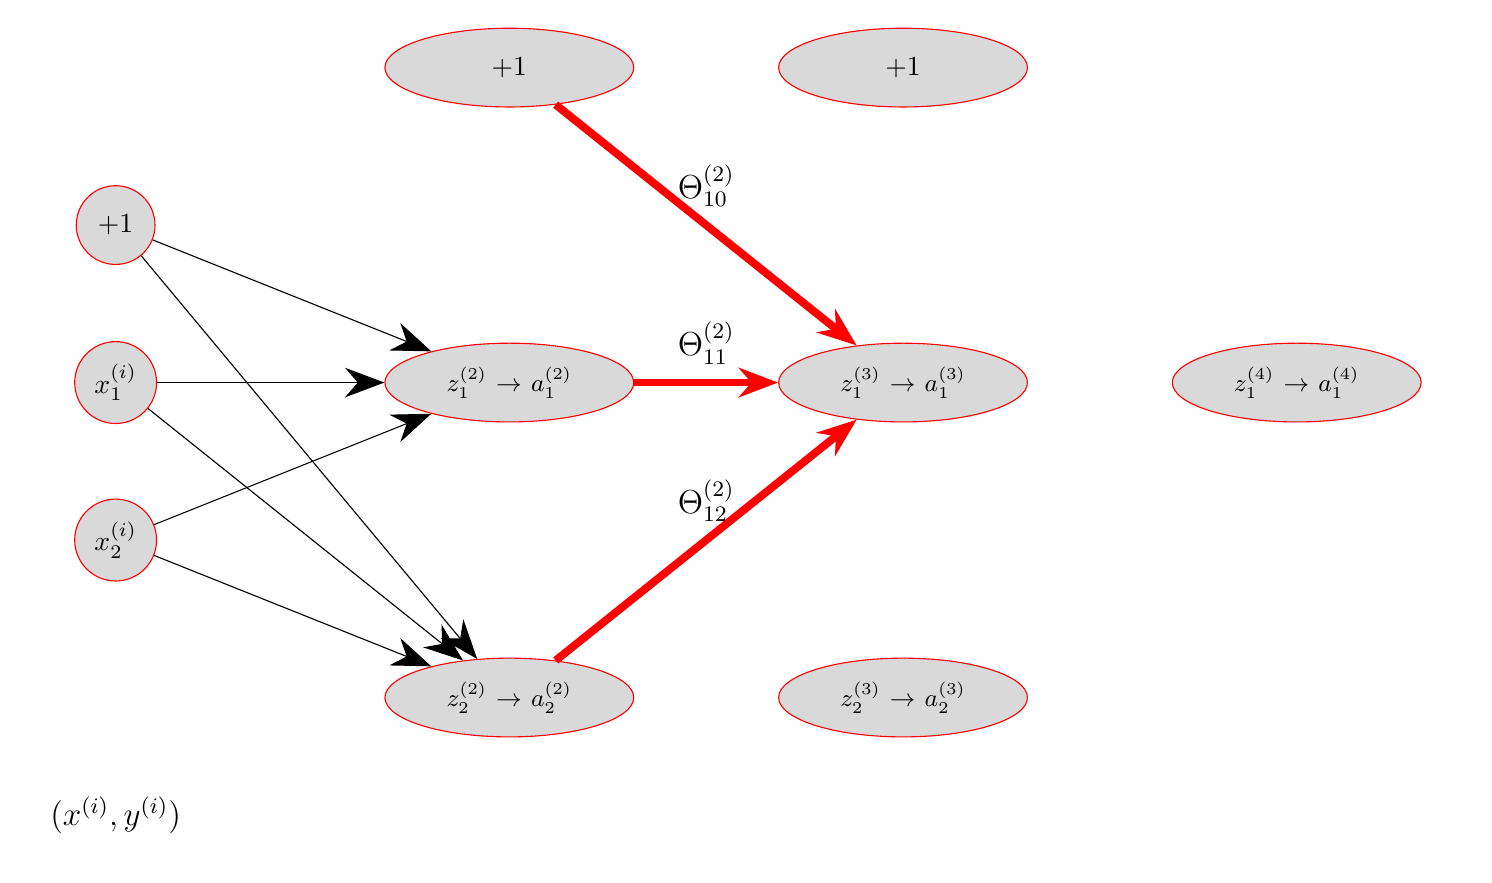
\begin{tikzpicture}[node distance=4cm]
\node (x1) [neuron] {+1};
\node (x2) [neuron, below of=x1, xshift=0cm, yshift=2cm] {$x_1 ^{(i)}$};
\node (x3) [neuron, below of=x2, xshift=0cm, yshift=2cm] {$x_2 ^{(i)}$};
\node (layer1) [smalldetail, below of=x2, xshift=0cm, yshift=-1.5cm] {\large{$(x^{(i)}, y^{(i)} )$}};
\node (a11) [neuronEll, below of=x1, xshift=5cm, yshift=6cm] {+1};
\node (a12) [neuronEll, below of=a11, xshift=0cm, yshift=0cm] {\small{$z_1^{(2)} \rightarrow a_1^{(2)}$}};
\node (a13) [neuronEll, below of=a12, xshift=0cm, yshift=0cm] {\small{$z_2^{(2)} \rightarrow a_2^{(2)}$}};
\node (layer2) [largedetail, below of=layer1, xshift=5cm, yshift=4cm] {};
\node (a21) [neuronEll, below of=a11, xshift=5cm, yshift=4cm] {+1};
\node (a22) [neuronEll, below of=a21, xshift=0cm, yshift=0cm] {\small{$z_1^{(3)} \rightarrow a_1^{(3)}$}};
\node (a23) [neuronEll, below of=a22, xshift=0cm, yshift=0cm] {\small{$z_2^{(3)} \rightarrow a_2^{(3)}$}};
\node (layer3) [largedetail, below of=layer2, xshift=5cm, yshift=4cm] {};
\node (a31) [neuronEll, below of=a21, xshift=5cm, yshift=0cm] {\small{$z_1^{(4)} \rightarrow a_1^{(4)}$}};
\node (layer4) [largedetail, below of=layer3, xshift=5cm, yshift=4cm] {};
\draw [-{Stealth[length=5mm]}] (x1) -- (a12);
\draw [-{Stealth[length=5mm]}] (x1) -- (a13);
\draw [-{Stealth[length=5mm]}] (x2) -- (a12);
\draw [-{Stealth[length=5mm]}] (x2) -- (a13);
\draw [-{Stealth[length=5mm]}] (x3) -- (a12);
\draw [-{Stealth[length=5mm]}] (x3) -- (a13);
\draw [-{Stealth[length=5mm]}][line width=1mm, red ] (a11) -- (a22);
\draw [-{Stealth[length=5mm]}][line width=1mm, red ] (a12) -- (a22);
\draw [-{Stealth[length=5mm]}][line width=1mm, red ] (a13) -- (a22);
\node (theta10) [smalldetail, below of=a11, xshift=2.5cm, yshift=2.5cm] {\large{$\Theta^{(2)}_{10}$}};
\node (theta11) [smalldetail, below of=theta10, xshift=0cm, yshift=2cm] {\large{$\Theta^{(2)}_{11}$}};
\node (theta12) [smalldetail, below of=theta11, xshift=0cm, yshift=2cm] {\large{$\Theta^{(2)}_{12}$}};
\end{tikzpicture}
}
\end{figure}
If we consider node 2 in layer 3: 
\begin{equation}
z_1 ^{(3)} = \Theta_{10} ^{(2)} \times 1 + \Theta_{11} ^{(2)} \times a_1 ^{(2)} + \Theta_{12} ^{(2)} \times a_1 ^{(2)}
\end{equation}
We can then apply the activation function to $z_1 ^{(3)}$ to get the activation value $a_1 ^{(3)}$.

\subsection{Back Propagation}
If we assume $\lambda = 0$, the cost function for a system with 1 output is defined by:
\begin{align*}
J(\theta) = -\frac{1}{m} \left[\sum_{i=1}^m y^{(i)} \mathrm{log}(h_{\theta}(x^{(i)})) + (1- y^{(i)}) \mathrm{log}(1-h_{\theta}(x^{(i)}))\right]
\end{align*}
For a single training example $(x^{i}, y^{i})$, the cost is:
\begin{align*}
\mathrm{cost}(i) = y^{(i)} \mathrm{log}(h_{\theta}(x^{(i)})) + (1- y^{(i)}) \mathrm{log}(1-h_{\theta}(x^{(i)}))
\end{align*}
We can think of $\mathrm{cost}(i)$ as being approximately the square error: $\mathrm{cost}(i) \approx (h_{\Theta}(x^{(i)} - y^{(i)})^2$. The cost is a measure of how well is the network doing on example $(i)$. \\
\textbf{Back propagation} is computing $\delta_j ^{(l)}$, the error of activation value calculated for unit $j$ in $l^{\mathrm{th}}$ layer. Formally (for $j \geq 0$):
\begin{align*}
\delta_j ^{(l)} = \frac{\partial }{\partial z_{j}^{(l)}} \mathrm{cost}(i)
\end{align*}

\begin{figure}[H]
\centering
\resizebox {5in} {!} {
\begin{tikzpicture}[node distance=4cm]
\node (x1) [neuron] {+1};
\node (x2) [neuron, below of=x1, xshift=0cm, yshift=2cm] {$x_1 ^{(i)}$};
\node (x3) [neuron, below of=x2, xshift=0cm, yshift=2cm] {$x_2 ^{(i)}$};
\node (layer1) [smalldetail, below of=x2, xshift=0cm, yshift=-1.5cm] {\large{$(x^{(i)}, y^{(i)} )$}};
\node (a11) [neuronEll, below of=x1, xshift=5cm, yshift=6cm] {+1};
\node (a12) [neuronEll, below of=a11, xshift=0cm, yshift=0cm] {$\delta_1 ^{(2)}$};
\node (a13) [neuronEll, below of=a12, xshift=0cm, yshift=0cm] {$\delta_2 ^{(2)}$};
\node (layer2) [largedetail, below of=layer1, xshift=5cm, yshift=4cm] {};
\node (a21) [neuronEll, below of=a11, xshift=5cm, yshift=4cm] {+1};
\node (a22) [neuronEll, below of=a21, xshift=0cm, yshift=0cm] {$\delta_1 ^{(3)}$};
\node (a23) [neuronEll, below of=a22, xshift=0cm, yshift=0cm] {$\delta_2 ^{(3)}$};
\node (layer3) [largedetail, below of=layer2, xshift=5cm, yshift=4cm] {};
\node (a31) [neuronEll, below of=a21, xshift=5cm, yshift=0cm] {$\delta_1 ^{(4)} = y^{(i)}-a_1^{(4)}$};
\draw [-{Stealth[length=5mm]}] (x1) -- (a12);
\draw [-{Stealth[length=5mm]}] (x1) -- (a13);
\draw [-{Stealth[length=5mm]}] (x2) -- (a12);
\draw [-{Stealth[length=5mm]}] (x2) -- (a13);
\draw [-{Stealth[length=5mm]}] (x3) -- (a12);
\draw [-{Stealth[length=5mm]}] (x3) -- (a13);
\draw [-{Stealth[length=5mm]}] (x2) -- (a13);
\draw [-{Stealth[length=5mm]}] (x3) -- (a12);
\draw [-{Stealth[length=5mm]}] (x3) -- (a13);
\draw [-{Stealth[length=5mm]}][line width=1mm, red ] (a31) -- (a22);
\draw [-{Stealth[length=5mm]}][line width=1mm, red ] (a31) -- (a23);
\draw [-{Stealth[length=5mm]}][line width=1mm, red ] (a22) -- (a13);
\draw [-{Stealth[length=5mm]}][line width=1mm, red ] (a23) -- (a13);
\node (theta11) [smalldetail, below of=theta10, xshift=5cm, yshift=2cm] {\large{$\Theta^{(3)}_{11}$}};
\node (theta12) [smalldetail, below of=theta11, xshift=0cm, yshift=2cm] {\large{$\Theta^{(3)}_{12}$}};
\node (theta11) [smalldetail, below of=theta10, xshift=0cm, yshift=0cm] {\large{$\Theta^{(2)}_{12}$}};
\node (theta12) [smalldetail, below of=theta11, xshift=0cm, yshift=2cm] {\large{$\Theta^{(2)}_{22}$}};
\end{tikzpicture}
}
\end{figure}
The error terms can be written as :
\begin{align}
\begin{split}
\delta_2 ^{(2)} &= \Theta_{12} ^{(2)} \delta_1 ^{(3)} + \Theta_{22} ^{(2)} \delta_2 ^{(3)} *g'(z_{(2)}) \\
& \\
\delta_2 ^{(3)} &= \Theta_{12} ^{(3)} \delta_1 ^{(4)} *g'(z_2 ^{(3)}) \\
\end{split}
\end{align} 

\section{Implementation note}
In previous assignments, we used the following lines to get the optimum \textbf{theta}, where \textbf{fminunc()} was the optimization algorithm. This routine assumes \textbf{initialTheta}, \textbf{theta} and \textbf{gradient} are all vectors.
\begin{python}
function [jVal, gradient] = costFunction(theta);
optTheta = fminunc(@costFunction, initialTheta, options)
\end{python}
With Neural Network, gradient \textbf{D}, \textbf{theta} are not vectors but matrices, so we need to unroll those matrices into vectors. \\
\begin{itemize}
\item Let's take a NN with $s_1=10$ (units in layer1), $s_2=10$ (units in layer2), $s_3=10$ (units in layer3)
\item $\Theta ^{(1)} \in \mathbb{R}^{(10\times 11)}$ and $\Theta ^{(2)} \in \mathbb{R}^{(1\times 11)}$
\item $D^{(1)} \in \mathbb{R}^{(10\times 11)}$ and $D^{(2)} \in \mathbb{R}^{(1\times 11)}$
\item before sending $\Theta$ and $D$ to \textbf{fminunc}, we will unroll them: \\
\begin{python}
thetaVec = [Theta1(:), Theta2(:)];
DVec = [D1(:), D2(:)];
\end{python}
\item when the result of \textbf{theta} is sent back from \textbf{fminunc}, the cost and gradient needs to be calculated but with \textbf{theta} in a matrix format:\\
\begin{python}
Theta1 = reshape(thetaVec(1:110), 10,11));
Theta1 = reshape(thetaVec(111:121), 1,11));
\end{python}
\end{itemize}

\section{Gradient checking}
This section shows a method to calculate a numerical estimation of gradient descent.

\begin{figure}[H]
\begin{center}$
\begin{array}[m]{r|l}
	\centering
        \includegraphics[totalheight=3cm]{Jcost.png}
& 
\begin{array}[b]{rl}
	\frac{d}{d \theta} J(\theta) & \approx \frac{J(\theta+\epsilon) + J(\theta-\epsilon)}{2 \epsilon} \\
	& \mathrm{typically \  use \ } \epsilon=10^{-4} \\
	&\mathrm{Note \  that\ } \theta \in \mathbb{R} \\
\end{array}
\end{array}$
\end{center}
\end{figure}

\begin{itemize}
\item Octave implementation
\end{itemize}
For $\theta \in  \mathbb{R}^n$ is a vector (unrolled version) of $\Theta^{(1)}$, $\Theta^{(2)}$..., i.e $\theta = [\theta_1, \theta_2,...\theta_n$.
The partial derivatives are:
\begin{align}
\begin{split}
\frac{\partial }{\partial \theta_1} J(\theta) & \approx \frac{J(\theta_1+\epsilon, \theta_2, ..., \theta_n) - J(\theta_1-\epsilon, \theta_2, ..., \theta_n)}{2 \epsilon} \\
\frac{\partial }{\partial \theta_2} J(\theta) & \approx \frac{J(\theta_1, \theta_2+\epsilon, ..., \theta_n) - J(\theta_1, \theta_2-\epsilon, ..., \theta_n)}{2 \epsilon} \\
.. & ..... \\
.. & ... \\
\frac{\partial }{\partial \theta_n} J(\theta) & \approx \frac{J(\theta_1, \theta_2, ..., \theta_n+\epsilon) - J(\theta_1, \theta_2, ..., \theta_n-\epsilon)}{2 \epsilon} \\
\end{split}
\end{align}
\begin{tcolorbox}
\begin{python}
for i=1:n,
	thetaPlus = theta;
	thetaPlus(i) = thetaPlus(i) + EPSILON;
	thetaMinus = theta;
	thetaMinus(i) = thetaMinus(i) - EPSILON;
	gradApprox(i) = (J(thetaPlus) - J(thetaMinus))/(2*EPSILON);
end
\end{python}
\end{tcolorbox}

\begin{itemize}
\item We then check that gradApprox $\approx$ Dvec (Dvec from backprop)
\end{itemize}


\section{Random Initialization for NN}
We have typically been using \textbf{initialTheta=zeros(1,n)}, but for NN this does not work.
\begin{figure}[H]
\begin{center}$
\begin{array}[b]{r|l}
\resizebox {2in} {!} {
\begin{tikzpicture}[node distance=3cm]
\node (x0) [startstop, below of=x1, xshift=0cm, yshift=6cm] {+1};
\node (x1) [startstop] {$x_1$};
\node (x2) [startstop, below of=x1, xshift=0cm, yshift=0cm] {$x_2$};
\node (a01) [neuron, below of=x0, xshift=5cm, yshift=3cm] {+1};
\node (a11) [neuron, below of=a01, xshift=0cm, yshift=0cm] {$a_1^{(2)}$};
\node (a12) [neuron, below of=a11, xshift=0cm, yshift=0cm] {$a_2^{(2)}$};
\node (output) [neuron, below of=a11, xshift=5cm, yshift=3cm] {$a_1^{(3)}$};
\node (h) [startstop, below of=output, xshift=5cm, yshift=3cm] {$h_{\Theta}(x)$};
\draw [-{Stealth[length=5mm]}][line width=1mm, red ] (x0) -- (a11);
\draw [-{Stealth[length=5mm]}][line width=1mm, red ] (x0) -- (a12);
\draw [-{Stealth[length=5mm]}][line width=1mm, green ] (x1) -- (a11);
\draw [-{Stealth[length=5mm]}][line width=1mm, green ] (x1) -- (a12);
\draw [-{Stealth[length=5mm]}][line width=1mm, blue ] (x2) -- (a11);
\draw [-{Stealth[length=5mm]}][line width=1mm, blue ] (x2) -- (a12);
\draw [-{Stealth[length=5mm]}] (a01) -- (output);
\draw [-{Stealth[length=5mm]}] (a11) -- (output);
\draw [-{Stealth[length=5mm]}] (a12) -- (output);
\draw [-{Stealth[length=5mm]}] (output) -- (h);
\end{tikzpicture} }
& 
\begin{array}[b]{rl}
&\mathrm{If \ } \Theta_{ij} ^{(l)} = 0 \mathrm{\ for all \ } i,j,l  \\
&\rightarrow a_1 ^{(2)} = a_2 ^{(2)} \\
&\rightarrow \delta_1 ^{(2)} = \delta_2 ^{(2)} \\
&\rightarrow \frac{\partial }{\partial \Theta_{01} ^{(1)}} J(\Theta)= \frac{\partial }{\partial \Theta_{02} ^{(1)}} J(\Theta) \\
&\rightarrow \mathrm{so \ even \ after \ 1 \ gradient \ descent \ update} \mathrm{new\_} \Theta_{01} ^{(1)} = \mathrm{new\_} \Theta_{02} ^{(1)} \\
&\rightarrow \mathrm{new\_} a_1 ^{(2)} = \mathrm{new\_} a_2 ^{(2)} \\
&\mathrm{This \ is \ the \ problem \ of \ weight \ symmetry} \\
\end{array}
\end{array}$
\end{center}
\end{figure}
For NN, we use random \textbf{initialTheta} to break the symmetry: i.e initialize each $\Theta_{ij}^{(l)}$ to a random value in $[-\epsilon, \epsilon]$ (small value close to 0).
\begin{tcolorbox}
\begin{python}
Theta1 = rand(10,11) \times (2 \times INIT_EPSILON) - INIT_EPSILON\end{python}
\end{tcolorbox}
This creates a (10,11) matrix with values between 0 and 1.

\begin{itemize}
\item Typically $\epsilon$ number is based on the different units in the network:
\begin{align}
\epsilon = \frac{\sqrt{6}}{\sqrt{L_{in} + L_{out}}}
\end{align}
where $L_{in}=s_l$ and $L_{out} =s_{l+1}$, i.e the number of units adjacent to $\Theta^{(l)}$
\end{itemize}
\section{Summary of NN implementation}
\begin{enumerate}
\item \textbf{Pick a network architecture}
	\begin{itemize}
	\item Nbr of input units (=Nbr of features) is set by the problem
	\item Nbr of output units (=Nbr of classes) is set by the problem
	\item number of hidden layer: a reasonable default is 1 hidden layer or if $>$ 1, the hidden layers have same Nbr of units 
	\end{itemize}
\item \textbf{Training a Neural Network}
	\begin{itemize}
	\item randomly initialize weights
	\item implement forward propagation to get $h_{\Theta}(x^{(i)})$ for example $x^{(i)}$
	\item implement code to compute $J(\Theta)$ 
	\item implement backprop to compute $\frac{\partial}{\partial \Theta_{ij} ^{(l)}} J(\Theta)$ 
	\end{itemize}
This is done with a for-loop:
\begin{tcolorbox}
\begin{python}
for i = 1:m 
	%Perform forward propagation and backprop on exampel i
	%get activations a(l) and delta(l)
	for l = 2:L
		Delta^(l) = Delta^(l) + delta^(l+1) Transpose[(a^(l))]
	
	end
end
...
%Compute partial derivative
\end{python}
\end{tcolorbox}

\item \textbf{Use gradient checking} \\
	\begin{itemize}
	\item compare numerical estimate of gradient of $J(\Theta)$ with $\frac{\partial}{\partial \Theta_ij ^{l}} J(\Theta)$ (from backprop)
	\item Disable gradient checking
	\end{itemize}
 
\item Use gradient descent or advanced optimization method (fminunc, etc..) with backprop to try to minimize $J(\Theta)$ as a function of $\Theta$
	\begin{itemize}
	\item compute $\frac{\partial }{\partial \Theta_ij ^{(l)}} J(\Theta)$
	\end{itemize}
for NN, $J(\Theta)$ is not convex, and gradient descent or other minimization algorithm can in theory be stucked in local minimum.
\end{enumerate}


\begin{appendices}
\section{Derivation of the node error term $\delta$}
\begin{itemize}
\item We know that for a logistic regression classifier, the cost function is defined as:
\end{itemize}
\begin{align}
J(\Theta) = -y \mathrm{log}[h_{\Theta})(x)] - (1-y)\mathrm{log}[1- h_{\Theta}(x)]
\end{align}
applied over the $K$ output neurons, and for all m examples.
\begin{itemize}
\item The partial derivatives of $J(\Theta)$ over the $\Theta$ in the output layer $(\partial J(\Theta) / \partial \Theta)$ is:
\end{itemize}
\begin{align}
\frac{\partial J(\Theta)}{\partial \Theta^{(L-1)}} = \frac{\partial J(\Theta)}{\partial a^{(L)}}\frac{\partial a^{(L)}}{\partial z^{(L)}} \frac{\partial z^{(L)}}{\partial \Theta^{(L-1)}}
\end{align}
\begin{itemize}
\item The partial derivatives of $J(\Theta)$ over the $\Theta$ in the last hidden layer $(\partial J(\Theta) / \partial \Theta)$ is:
\end{itemize}
\begin{align}
\frac{\partial J(\Theta)}{\partial \Theta^{(L-2)}} = \frac{\partial J(\Theta)}{\partial a^{(L)}}\frac{\partial a^{(L)}}{\partial z^{(L)}} \frac{\partial z^{(L)}}{\partial \Theta^{(L-1)}}\frac{\partial a^{(L-1)}}{\partial z^{(L-1)}}\frac{\partial z^{(L-1)}}{\partial \Theta^{(L-2)}}
\end{align}
\begin{itemize}
\item Clearly the output layer and the hidden layer immediately before it share some pieces in common, which we denotes $\delta ^{(L)}$, the error node
\end{itemize}
\begin{align}
\delta^{(L)} =  \frac{\partial J(\Theta)}{\partial a^{(L)}}\frac{\partial a^{(L)}}{\partial z^{(L)}}
\end{align}
\begin{itemize}
\item Similarly $\delta ^{(L-1)}$ would be the pieces shared by the final hidden layer ($L-1$) and a hidden layer before it ($L-2$):
\end{itemize}
\begin{align}
\begin{split}
\delta^{(L-1)} &=  \frac{\partial J(\Theta)}{\partial a^{(L)}}\frac{\partial a^{(L)}}{\partial z^{(L)}}\frac{\partial z^{(L)}}{\partial a^{(L-1)}}\frac{\partial a^{(L-1)}}{\partial z^{(L-1)}} \\
&=\delta^{(L)} \frac{\partial z^{(L)}}{\partial a^{(L-1)}}\frac{\partial a^{(L-1)}}{\partial z^{(L-1)}}
\end{split}
\end{align}
\begin{itemize}
\item With this $\delta$-terms, our equations become:
\end{itemize}
\begin{align}
\begin{split}
\frac{\partial J(\Theta)}{\partial \Theta^{(L-1)}} &=  \delta^{(L)}\frac{\partial z^{(L)}}{\partial a^{(L-1)}}\\
\frac{\partial J(\Theta)}{\partial \Theta^{(L-2)}} &= \delta^{(L-1)} \frac{\partial z^{(L-1)}}{\partial a^{(L-2)}}
\end{split}
\end{align}
Now we evaluate those derivatives:
\begin{itemize}
\item Let's start with the output layer:
\end{itemize}
\begin{align}
\begin{split}
\frac{\partial J(\Theta)}{\partial \Theta^{(L-1)}} =  \delta^{(L)}\frac{\partial z^{(L)}}{\partial a^{(L-1)}}\\
\end{split}
\end{align}
Using $\delta^{(L)} = \frac{\partial J(\Theta}{\partial a^{(L)}}{\partial z^{(L)}}$ and $J(\Theta) = -y \mathrm{log}[a^{(L)}] - (1-y)\mathrm{log}[1-a^{(L)}]$ where $a^{(L)}=h_{\Theta}(x)$, we get:
\begin{align}
\frac{\partial J(\Theta)}{\partial a^{(L)}} = \frac{y-1}{a^{(L)}-1} - \frac{y}{a^{(L)}}
\end{align}
and given $a=g(z)$, where $g=\frac{1}{1+e^{-z}}$:
\begin{align}
\frac{\partial a^{(L)}}{\partial z^{(L)}} = a^{(L)}(1- a^{(L)})
\end{align}
\begin{itemize}
\item We now substitute in the definition of $\delta^{(L)}$:
\end{itemize}
\begin{align}
\begin{split}
\delta^{(L)} &= \frac{\partial J(\Theta)}{\partial a^{(L)}}\frac{\partial a^{(L)}}{\partial z^{(L)}} = \left( \frac{y-1}{a^{(L)}-1} - \frac{y}{a^{(L)}}\right) ( a^{(L)}(1-a^{(L)})) \\
&= a^{(L)} - y
\end{split}
\end{align}
\begin{itemize}
\item Given $z=\Theta * input $  where in layer $L$, the input is $a^{(L-1)}$:
\end{itemize}
\begin{align}
\begin{split}
\frac{\partial z^{(L)}}{\partial \Theta^{(L-1)}} &= \delta^{(L)}\frac{\partial z^{(L)}}{\partial \Theta^{(L-1)}}\\
&= (a^{(L)}-y)a^{(L-1)}
\end{split}
\end{align}

\begin{itemize}
\item Let's run the calculation for the hidden layer $\frac{\partial J(\theta)}{\partial \theta^{(L-2)}} = \delta^{(L-1)} \frac{\partial z^{(L-1)}}{\partial \Theta^{(L-2)}}$ (we assume we have 1 hidden layer):
\end{itemize}
Once again, given $z=\Theta*input$:
\begin{align}
\begin{split}
\frac{\partial z^{(L)}}{\partial a^{(L-1)}} &= \Theta^{(L-1)} \\
\frac{\partial a^{(L-1)}}{\partial z^{(L-1)}} &= a^{(L-1)} (1-a^{(L-1)}
\end{split}
\end{align}
\begin{itemize}
\item We then substitute in $\delta^{(L-1)}$
\end{itemize}
\begin{align}
\begin{split}
\delta^{(L-1)} &= \delta^{(L)}\frac{\partial z^{(L)}}{\partial a^{(L-1)}} \frac{\partial a^{(L-1)}}{\partial z^{(L-1)}} \\
&=\delta^{(L)} \Theta^{(L-1)}(a^{(L-1)}(1- a^{(L-1)}))
\end{split}
\end{align}
\begin{itemize}
\item So, for a 3 layer network:
\end{itemize}
\begin{align}
\delta^{(2)} = \delta^{(2)} \Theta^{(2)}(a^{(2)}(1- a^{(2)}))
\end{align}
\begin{itemize}
\item The derivative of the cost function about the weights $\Theta$ in the last hidden layer:
\end{itemize}
\begin{align}
\begin{split}
\frac{\partial J(\Theta)}{\partial \Theta ^{(L-2)}} &= \delta^{(L-1)} \frac{\partial z^{(L-1)}}{\partial \Theta^{(L-2)}} \\
&= (\delta^{(L)} \frac{\partial z^{(L)}}{\partial a^{(L-1)}} \frac{\partial a^{(L-1)}}{\partial z^{(L-1)}})a^{(L-2)} \\
&=((a^{(L)}-y)(\Theta^{(L-1)})(a^{(L-1)}(1-a^{(L-1)})))(a^{(L-2)})
\end{split}
\end{align}

Derivative $g'(z)$:
\begin{align}
\begin{split}
g(z)' =& (\frac{1}{1+ e^{-z}})' = -\frac{-e^{-z}}{(1+ e^{-z})^2} = \frac{e^{-z}}{(1+ e^{-z})} g(z) = \frac{1-1+e^{-z}}{(1+ e^{-z})} g(z) \\
 =& (1 - \frac{1}{(1+ e^{-z})}) g(z) = (1 - g(z)) g(z)
\end{split}
\end{align}

\section{links}
%http://neuralnetworksanddeeplearning.com/chap3.html\#the_cross-entropy\_cost\_function

\section{Good to know}
\begin{itemize}
\item The Hadamard or Schur product denotes "element-wise" product of 2 matrices:
\begin{equation}
s \odot t
\end{equation}

\item An alternative to logistic function (sigmoid) is :
\begin{align*}
g(x) = \mathrm{tanh}(x)
\end{align*}

\item Cross entropy cost function ???
\end{itemize}

\end{appendices}
\end{document}